\documentclass{beamer}
\usepackage[orientation=portrait,size=a0,scale=1.4,debug]{beamerposter}
\mode<presentation>{\usetheme{ZH}}
\usepackage[T1]{fontenc}
\usepackage[utf8]{inputenc}
\usepackage{siunitx} %pretty measurement unit rendering
\usepackage{hyperref} %enable hyperlink for urls
\usepackage{ragged2e}
\usepackage{amsthm,amsmath,amsfonts,exscale,latexsym}
\usepackage{pmboxdraw}
\usepackage{newunicodechar}
\usepackage{natbib, times}
\newunicodechar{─}{\textSFx}
\newunicodechar{μ}{$\mu$}
\newunicodechar{ω}{$\omega$}
\newunicodechar{β}{$\beta$}
\newunicodechar{α}{$\alpha$}
\newunicodechar{₁}{\textsubscript{1}}
\usepackage[usefamily={juliacon, julia}, autoprint=false]{pythontex}

\usepackage[font=scriptsize,justification=justified]{caption}
\usepackage{array,booktabs,tabularx}
\newcolumntype{Z}{>{\centering\arraybackslash}X} % centered tabularx columns
\sisetup{per=frac,fraction=sfrac}

\title{\huge \texttt{ARCHModels.jl}}
\author{Simon A.\ Broda}
\institute[UZH]{University of Zurich }
\date{\today}

% edit this depending on how tall your header is. We should make this scaling automatic :-/
\newlength{\columnheight}
\setlength{\columnheight}{104cm}

\begin{document}
\begin{frame}[fragile]
\begin{columns}
\begin{column}{.48\textwidth}
\begin{beamercolorbox}[center]{postercolumn}
\begin{myblock}{Introduction}
\begin{juliacode}
using Pkg
Pkg.add(["BenchmarkTools", "Plots", "MATLAB",
             "MarketData", "TimeSeries", "Distributions",
             "KernelDensity", "StatsPlots", "ProgressMeter"
#             ,"ARCHModels"
])
pkg"precompile"
using MarketData, TimeSeries
r = percentchange(MarketData.AAPL[Symbol("Adj. Close")]) # returns a TimeSeries
data = values(r) # an array containing just the plain data

if !isfile(joinpath("img", "returns.pdf")) || !isfile(joinpath("img", "kde.pdf"))
    using Plots, Distributions, KernelDensity, StatsPlots
    plot(r, title="Volatility Clustering", legend=:none, ylabel="\$r_t\$")
    savefig(joinpath("img", "returns.pdf"))
    plot(kde(data), label="Kernel Density", title="Fat Tails")
    plot!(fit(Normal, data), label="Fitted Normal")
    savefig(joinpath("img", "kde.pdf"))
end
\end{juliacode}
\begin{itemize}
\item Daily financial returns data exhibit a number of {\color{red}stylized facts}:
\begin{itemize}
  \item Volatility clustering
  \item Non-Gaussianity, fat tails
  \item Leverage effects: negative returns have larger effect on future volatility
\end{itemize}
\item Similar for other data (e.g., changes in interest rates).
\item Important throughout finance (risk management, derivative pricing, portfolio management, \ldots).
\item {}[G]ARCH ([{\bf G}eneralized] {\bf A}utoregressive {\bf C}onditional {\bf V}olatility) models are the most popular for modelling them.
\end{itemize}
\vspace{1em}

\begin{tabular}{cc}
\multicolumn{2}{c}{\bf Example: AAPL}\\
\IfFileExists{img/returns.pdf}{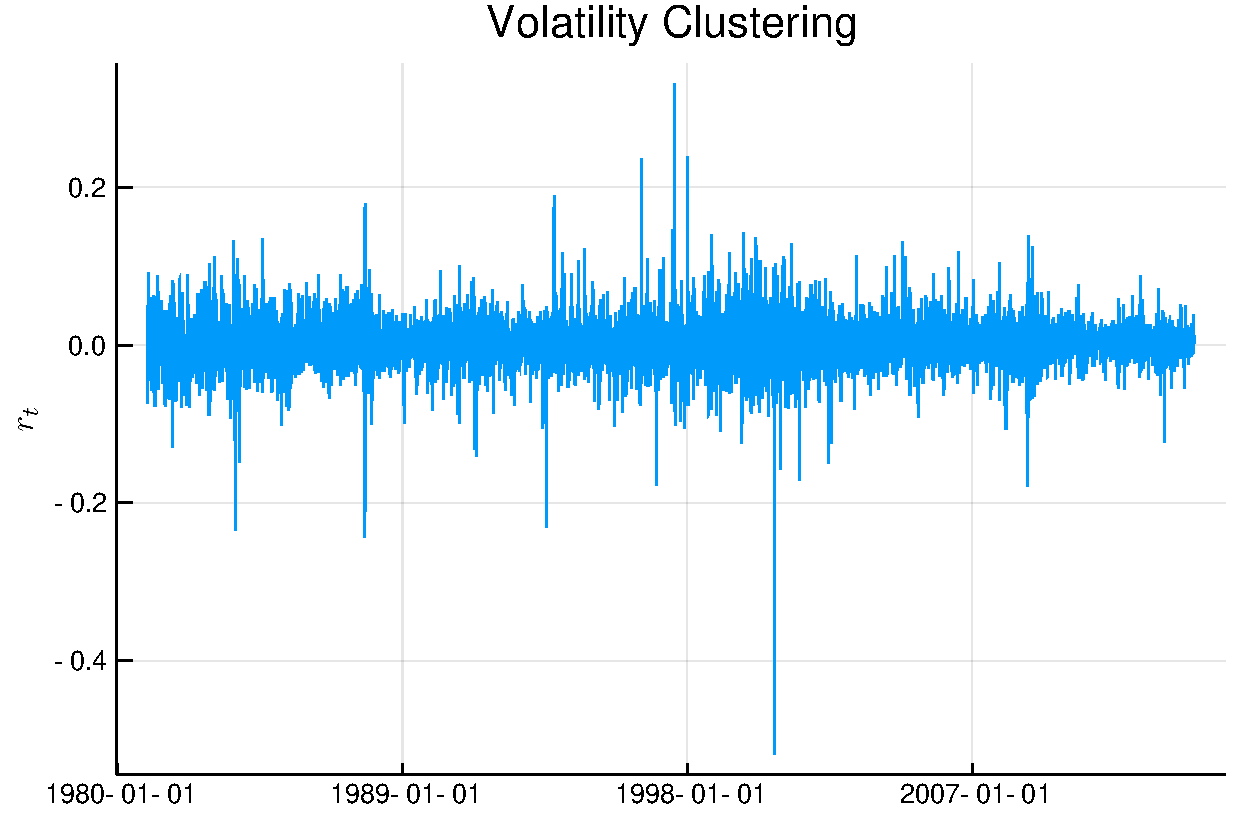
\includegraphics[width=0.45\textwidth]{img/returns}}{} &
\IfFileExists{img/kde.pdf}{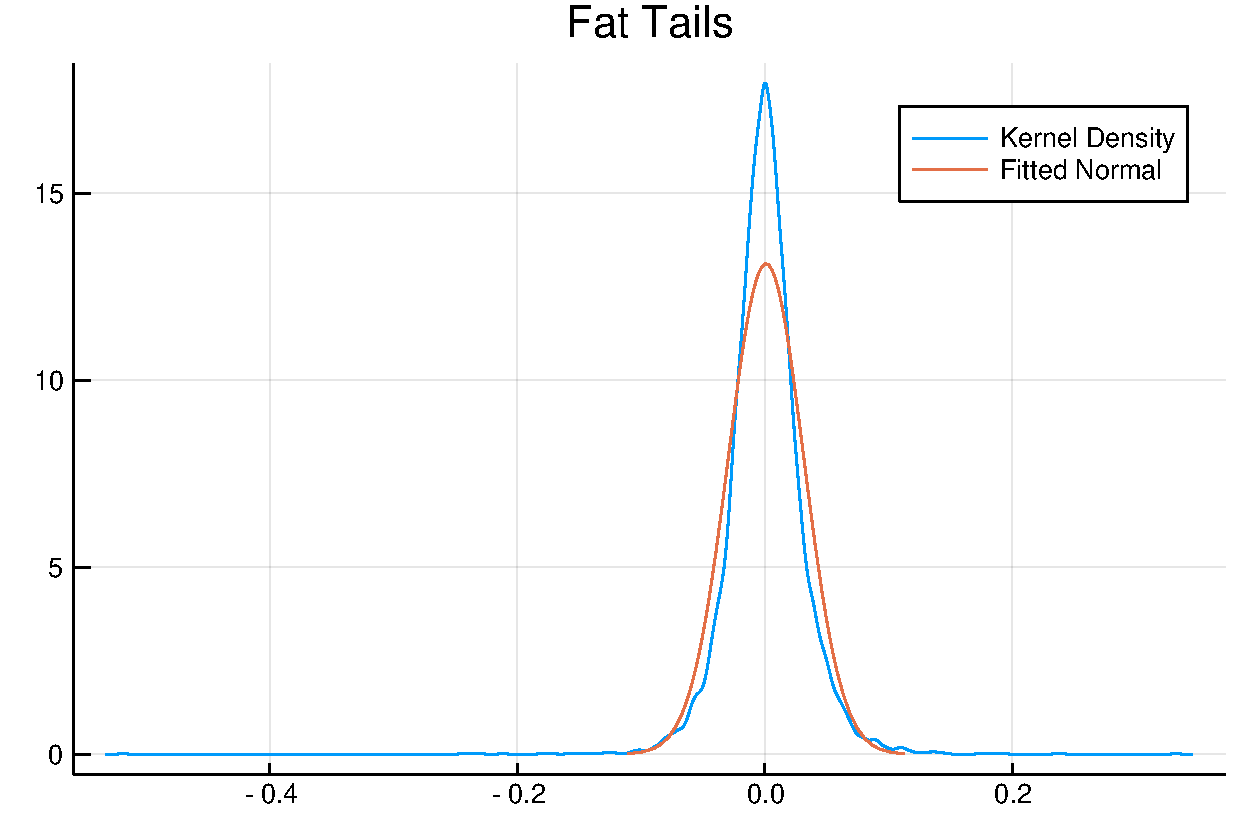
\includegraphics[width=0.45\textwidth]{img/kde}}{}
\end{tabular}

\end{myblock}\vfill
\begin{myblock}{[G]ARCH Models}
\begin{itemize}
\item Basic setup: given a sample of financial returns $\{r_t\}_{t\in\{1,\ldots,T\}}$, decompose $r_t$ as
\[
r_t=\mu_t+\sigma_tz_t, \quad z_t\stackrel{i.i.d.}{\sim}(0,1),
\]
where $\mu_t\equiv\mathbb{E}[r_t\mid \mathcal{F}_{t-1}]$ and $\sigma_t^2\equiv \mathbb{E}[(r_t-\mu_t)^2\mid \mathcal{F}_{t-1}]$.
\item Assume $\mu_t=0$ for simplicity. Focus is on the volatility $\sigma_t$.
\item {}[G]ARCH models make $\sigma_t$ a function of \emph{past} returns and variances. Examples:
\begin{itemize}
\item ARCH(q) \citep{en:82}:
\[
\sigma_t^2=\omega+\sum_{i=1}^q \alpha_ir_{t-i}^2%,\quad \omega,\alpha_i>0,\quad \sum_{i=1}^q\alpha_i<1.
\]
\item {\color{red}GARCH(p, q)} \citep{bo:86}:
\[
\sigma_t^2=\omega+ \sum_{i=1}^p\beta_{i}\sigma_{t-i}^2 + \sum_{i=1}^q\alpha_ir_{t-i}^2%,\quad \omega,\alpha_i,\beta_i>0,\quad \sum_{i=1}^{\max p,q} \alpha_i+\beta_i<1.
\]
\item TGARCH \citep{gjr:93}:
\[
\sigma_t^2=\omega+\sum_{i=1}^o\gamma_i  a_{t-i}^2 1_{a_{t-i}<0}+\sum_{i=1}^p\beta_i \sigma_{t-i}^2+\sum_{i=1}^q\alpha_i a_{t-i}^2.% \quad \omega, \alpha_i, \beta_i, \gamma_i>0, \sum_{i=1}^{\max o,p,q} \alpha_i+\beta_i+\gamma_i/2<1.
\]
\item EGARCH(o, p, q) \citep{ne:91}:
\[
\log(\sigma_t^2)=\omega+\sum_{i=1}^o\gamma_{i}z_{t-i}+\sum_{i=1}^p\beta_i\log(\sigma_{t-i}^2)+\sum_{i=1}^q \alpha_i (|z_t|-\mathbb{E}|z_t|)%, \quad \sum_{i=1}^p \beta_i<0.
\]
\end{itemize}
\end{itemize}
\end{myblock}\vfill
\begin{myblock}{Estimation}
\begin{itemize}
\item {}[G]ARCH models are usually estimated by maximum likelihood: with $f_z$ denoting the density of $z_t$,
\[\max \prod_t f(r_t\mid \mathcal{F}_{t-1})=\max \prod_t\frac{1}{\sigma_t}f_z(r_t/\sigma_t).\]
\item {\color{red}$\sigma_t$ is recursive} $\Rightarrow$ not ``vectorizable'' $\Rightarrow$ {\color{red}loops}.
\item Matlab, Python's \texttt{rugarch} have to implement the likelihood in C.
\end{itemize}
\end{myblock}\vfill
\begin{myblock}{\texttt{ARCHModels.jl} Highlights}
\begin{itemize}
\item \texttt{ARCHModels.jl} is registered and supports Julia 1.0 and later.
\item Extensive documentation available at \url{https://s-broda.github.io/ARCHModels.jl/stable/}.
\item Implements estimation and inference for ARCH, GARCH, TGARCH, and EGARCH models of arbitrary orders.
\item Supports Gaussian, GED, and Student's $t$ errors natively, plus {\color{red}any} continuous distribution from \texttt{Distributions.jl}.
\item Mean equations can be specified as {\color{red}ARMA(p, q)} models, or a {\color{red}regression model} from \texttt{GLM.jl}.
\item Also: automatic model selection, risk measure calculation, forecasting, simulation, model diagnostics, specification tests.
\item Most importantly, it's\\\Centering {\color{ETH10}\bf\scshape Faaaaaaaaaaaast!}
\end{itemize}
\end{myblock}\vfill
\end{beamercolorbox}
\end{column}



\begin{column}{.48\textwidth}
\begin{beamercolorbox}[center]{postercolumn}
\begin{myblock}{Implementation}
\begin{itemize}
\item Designed to be easily {\color{red}extensible} with new models, distributions.
\item Volatility specifications subtype \texttt{VolatilitySpec}. Parametrized on $(o, p, q)$ to facilitate loop unrolling.
\item Simulation and estimation return instances of \texttt{UnivariateARCHModel}, which implements \texttt{StatisticalModel} from \texttt{StatsBase}.
\item ML estimation via \texttt{Optim.jl}, standard errors obtained by AD via \texttt{ForwardDiff.jl}.
\end{itemize}
\end{myblock}\vfill

\begin{myblock}{Benchmarks}
{\footnotesize
\begin{juliaconsole}
using ARCHModels, MATLAB, BenchmarkTools
mat"version"
@btime fit(GARCH{1, 1}, $BG96, meanspec=NoIntercept)
mat"tic; estimate(garch(1, 1), $BG96); toc; 0";
\end{juliaconsole}
}
\end{myblock}\vfill

%\begin{myblock}{Further Usage Examples}
%\begin{itemize}

%\end{itemize}
%{\footnotesize
%\begin{juliaconsole}
%using ARCHModels
%fit(GARCH{1, 1}, BG96)
%\end{juliaconsole}
%}
%\end{myblock}\vfill
\begin{myblock}{Results}
\begin{itemize}
\item \texttt{BG96} are daily DM/GBP exchange rate data from \citet{bg:96}, the de-facto standard for testing implementations of [G]ARCH models.
\item \texttt{ARCHModels.jl} beats Matlab by a {\color{red} factor of about 10}, despite Matlab implementing the likelihood {\color{red}in C}.
\item Estimates are similar, but standard errors and $t$-stats are not.
\item \texttt{ARCHModels.jl} {\color{red}matches} the benchmark results given in \citet{bbp:01} to the published precision.
\end{itemize}
\end{myblock}
\begin{myblock}{References}
\footnotesize
\bibliographystyle{biometrika}
\bibliography{./bib}
\end{myblock}\vfill
\begin{myblock}{Acknowledgement}
This project has received funding from the European Research Council (ERC) under the European Union's Horizon 2020 research and innovation  program (grant agreement No. 750559).
\end{myblock}\vfill
\end{beamercolorbox}
\end{column}
\end{columns}
\end{frame}
\end{document}
